% SEDS500 Project Defense Presentation
% Privacy-Preserving Synthetic Tabular Data Generation Using Diffusion Models
% Author: Umut Akın
% Date: January 2026

\documentclass[aspectratio=169,11pt]{beamer}

% Theme - Dracula
\usetheme{Madrid}
\usecolortheme{default}

% Dracula color palette
\definecolor{draculabg}{RGB}{40, 42, 54}
\definecolor{draculacurrent}{RGB}{68, 71, 90}
\definecolor{draculafg}{RGB}{248, 248, 242}
\definecolor{draculacomment}{RGB}{98, 114, 164}
\definecolor{draculacyan}{RGB}{139, 233, 253}
\definecolor{draculagreen}{RGB}{80, 250, 123}
\definecolor{draculaorange}{RGB}{255, 184, 108}
\definecolor{draculapink}{RGB}{255, 121, 198}
\definecolor{draculapurple}{RGB}{189, 147, 249}
\definecolor{draculared}{RGB}{255, 85, 85}
\definecolor{draculayellow}{RGB}{241, 250, 140}

% Apply Dracula theme
\setbeamercolor{background canvas}{bg=draculabg}
\setbeamercolor{normal text}{fg=draculafg}
\setbeamercolor{structure}{fg=draculapurple}
\setbeamercolor{frametitle}{bg=draculacurrent,fg=draculafg}
\setbeamercolor{title}{fg=draculafg}
\setbeamercolor{subtitle}{fg=draculacyan}
\setbeamercolor{title separator}{fg=draculapurple}
\setbeamercolor{palette primary}{bg=draculacurrent,fg=draculafg}
\setbeamercolor{palette secondary}{bg=draculacurrent,fg=draculafg}
\setbeamercolor{palette tertiary}{bg=draculapurple,fg=draculafg}
\setbeamercolor{palette quaternary}{bg=draculacurrent,fg=draculafg}
\setbeamercolor{titlelike}{parent=palette primary,fg=draculafg}
\setbeamercolor{author}{fg=draculafg}
\setbeamercolor{institute}{fg=draculacomment}
\setbeamercolor{date}{fg=draculacomment}
\setbeamercolor{item}{fg=draculacyan}
\setbeamercolor{block title}{bg=draculacurrent,fg=draculagreen}
\setbeamercolor{block body}{bg=draculabg,fg=draculafg}
\setbeamercolor{block title alerted}{bg=draculared,fg=draculafg}
\setbeamercolor{block body alerted}{bg=draculacurrent,fg=draculafg}
\setbeamercolor{alerted text}{fg=draculared}
\setbeamercolor{footline}{fg=draculacomment}
\setbeamercolor{section in toc}{fg=draculacyan}
\setbeamercolor{subsection in toc}{fg=draculafg}
\setbeamercolor{section number projected}{bg=draculapurple,fg=draculafg}
\setbeamercolor{subsection number projected}{bg=draculacurrent,fg=draculafg}

% Packages
\usepackage[utf8]{inputenc}
\usepackage[T1]{fontenc}
\usepackage{graphicx}
\usepackage{booktabs}
\usepackage{amsmath}
\usepackage{tikz}
\usepackage{colortbl}

% Table colors for dark theme
\arrayrulecolor{draculacomment}

% Graphics path
\graphicspath{{../figures/}}

% Remove navigation symbols
\setbeamertemplate{navigation symbols}{}

% Add slide numbers
\setbeamertemplate{footline}[frame number]

% Title information
\title[Synthetic Data via Diffusion]{Privacy-Preserving Synthetic Tabular Data Generation Using Diffusion Models}
\subtitle{SEDS500 Graduation Project}
\author{Umut Ak{\i}n}
\institute[IZTECH]{
    Izmir Institute of Technology\\
    Graduate School of Engineering and Sciences\\
    Department of Computer Engineering
}
\date{January 2026}

\begin{document}

% Title slide
\begin{frame}
    \titlepage
\end{frame}

% Outline - Staircase layout
\begin{frame}{Outline}
    \vspace{-0.5cm}
    \Large
    \begin{flushleft}
        \hspace{0.5cm}\textcolor{draculapurple}{\textbf{1}} \textcolor{draculacyan}{Abstract}\\[0.4cm]
        \hspace{2.0cm}\textcolor{draculapurple}{\textbf{2}} \textcolor{draculacyan}{Introduction}\\[0.4cm]
        \hspace{3.5cm}\textcolor{draculapurple}{\textbf{3}} \textcolor{draculacyan}{Related Research}\\[0.4cm]
        \hspace{5.0cm}\textcolor{draculapurple}{\textbf{4}} \textcolor{draculacyan}{Solution Approach}\\[0.4cm]
        \hspace{6.5cm}\textcolor{draculapurple}{\textbf{5}} \textcolor{draculacyan}{Validation Approach}\\[0.4cm]
        \hspace{8.0cm}\textcolor{draculapurple}{\textbf{6}} \textcolor{draculacyan}{Conclusion \& Future Work}
    \end{flushleft}
\end{frame}

%===============================================
\section{Abstract}
%===============================================

\begin{frame}{Abstract}
    \begin{block}{Research Summary}
        This project investigates \textbf{diffusion models} as a privacy-preserving approach for generating synthetic tabular data.
    \end{block}

    \vspace{0.3cm}
    \textbf{Method:} TabDDPM-style diffusion with hybrid Gaussian-Multinomial noise

    \vspace{0.3cm}
    \textbf{Comparison:} Against CTGAN (GAN-based) and SMOGN (interpolation-based)

    \vspace{0.3cm}
    \textbf{Key Results:}
    \begin{itemize}
        \item \textbf{87--98\%} of baseline model performance with synthetic data alone
        \item Significantly outperforms CTGAN (35\%) and SMOGN (fails completely)
        \item \textbf{Zero privacy leakage} (membership inference AUC = 0.51)
    \end{itemize}

    \vspace{0.3cm}
    \textbf{Conclusion:} Diffusion models are superior for generating high-utility, privacy-preserving synthetic tabular data.
\end{frame}

%===============================================
\section{Introduction}
%===============================================

\begin{frame}{Motivation: Data Sharing vs Privacy}
    \begin{columns}
        \column{0.05\textwidth}
        \column{0.45\textwidth}
        \textbf{Organizations want to:}
        \begin{itemize}
            \item Share data with partners
            \item Enable ML research
            \item Collaborate across teams
        \end{itemize}

        \vspace{0.5cm}
        \textbf{But they face:}
        \begin{itemize}
            \item Privacy regulations (GDPR, KVKK)
            \item Sensitive customer data
            \item Competitive concerns
        \end{itemize}

        \column{0.5\textwidth}
        \centering
        \textbf{Solution: Synthetic Data}

        \vspace{0.3cm}
        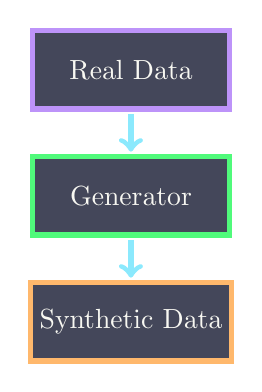
\begin{tikzpicture}[scale=0.8]
            \node[draw=draculapurple, line width=2pt, rectangle, fill=draculacurrent, text=draculafg, minimum width=2.5cm, minimum height=1cm] at (0,2) {Real Data};
            \draw[->, line width=2pt, draculacyan] (0,1.3) -- (0,0.7);
            \node[draw=draculagreen, line width=2pt, rectangle, fill=draculacurrent, text=draculafg, minimum width=2.5cm, minimum height=1cm] at (0,0) {Generator};
            \draw[->, line width=2pt, draculacyan] (0,-0.7) -- (0,-1.3);
            \node[draw=draculaorange, line width=2pt, rectangle, fill=draculacurrent, text=draculafg, minimum width=2.5cm, minimum height=1cm] at (0,-2) {Synthetic Data};
        \end{tikzpicture}

        \vspace{0.3cm}
        \small Same statistical properties,\\no original records exposed
    \end{columns}
\end{frame}

\begin{frame}{Problem Definition \& Goal}
    \begin{block}{Problem}
        Traditional synthetic data methods (interpolation, GANs) struggle with complex tabular data containing mixed numerical and categorical features.
    \end{block}

    \vspace{0.3cm}
    \begin{block}{Research Question}
        \centering
        When generating synthetic tabular data for privacy purposes,\\
        \textbf{do diffusion models produce more realistic data}\\
        than traditional methods?
    \end{block}

    \vspace{0.3cm}
    \textbf{Evaluation Criteria:}
    \begin{enumerate}
        \item \textbf{Utility}: Can ML models trained on synthetic data perform well on real data?
        \item \textbf{Privacy}: Does the synthetic data leak information about training records?
    \end{enumerate}
\end{frame}

\begin{frame}{Proposed Solution}
    \begin{center}
    \tikz{
        \node[fill=draculapurple, rounded corners=5pt, inner sep=10pt, text=draculafg] {
            \large\textbf{Implement TabDDPM-style diffusion for tabular data generation}
        };
    }
    \end{center}

    \vspace{0.3cm}
    \begin{columns}[t]
        \column{0.5\textwidth}
        \textbf{Key innovations:}
        \begin{itemize}
            \item Hybrid noise handling
            \item Gaussian for numerical features
            \item Multinomial for categorical features
            \item Log-space operations for stability
            \item KL divergence loss
        \end{itemize}

        \column{0.5\textwidth}
        \textbf{Methods compared:}
        \begin{itemize}
            \item \textbf{TabDDPM-style} (ours)
            \item CTGAN (GAN-based)
            \item SMOGN (interpolation)
        \end{itemize}

        \vspace{0.3cm}
        \textbf{Datasets:}
        \begin{itemize}
            \item Production (5,370 samples)
            \item Ozel Rich (2,670 samples)
        \end{itemize}
    \end{columns}
\end{frame}

%===============================================
\section{Related Research}
%===============================================

\begin{frame}{Related Research}
    \begin{table}
        \centering
        \small
        \begin{tabular}{llll}
            \toprule
            \textbf{Paper} & \textbf{Venue} & \textbf{Approach} & \textbf{Key Innovation} \\
            \midrule
            TabDDPM & ICML 2023 & Diffusion & Hybrid Gaussian-Multinomial noise \\
            CTGAN & NeurIPS 2019 & GAN & Mode-specific normalization \\
            STaSy & ICLR 2023 & Score-based & Self-paced learning \\
            TabSyn & ICLR 2024 & Latent diffusion & Transformer VAE encoder \\
            \bottomrule
        \end{tabular}
    \end{table}

    \vspace{0.3cm}
    \textbf{Why diffusion over GANs?}
    \begin{itemize}
        \item GANs suffer from mode collapse and training instability
        \item Diffusion models have stable training dynamics
        \item Iterative refinement captures full data distribution
    \end{itemize}

    \vspace{0.3cm}
    \textbf{Our contribution:} Implement and evaluate TabDDPM-style diffusion on real organizational datasets with privacy validation.
\end{frame}

%===============================================
\section{Solution Approach}
%===============================================

\begin{frame}{Diffusion Models: Core Idea}
    \begin{columns}
        \column{0.55\textwidth}
        \textbf{Forward Process (Training):}
        \begin{itemize}
            \item Gradually add noise to data
            \item Over $T=1000$ timesteps
            \item Data becomes pure noise
        \end{itemize}

        \vspace{0.3cm}
        \textbf{Reverse Process (Generation):}
        \begin{itemize}
            \item Learn to denoise step-by-step
            \item Neural network predicts noise
            \item Random noise $\rightarrow$ realistic data
        \end{itemize}

        \column{0.45\textwidth}
        \centering
        \includegraphics[width=\textwidth]{fig6_diffusion_process.png}
    \end{columns}

    \vspace{0.3cm}
    \textbf{Key advantage:} Stable training, captures full distribution (no mode collapse)
\end{frame}

\begin{frame}{TabDDPM: Handling Mixed Data Types}
    \textbf{Challenge:} Tabular data has both numerical and categorical features

    \vspace{0.5cm}
    \begin{columns}
        \column{0.5\textwidth}
        \textbf{Numerical Features:}
        \begin{itemize}
            \item Standard Gaussian diffusion
            \item Add/remove continuous noise
            \item Example: price, quantity
        \end{itemize}

        \column{0.5\textwidth}
        \textbf{Categorical Features:}
        \begin{itemize}
            \item Multinomial diffusion
            \item Transition between categories
            \item Example: product type, material
        \end{itemize}
    \end{columns}

    \vspace{0.5cm}
    \begin{block}{Hybrid Approach}
        \centering
        Process numerical and categorical features simultaneously\\
        with type-appropriate noise schedules
    \end{block}
\end{frame}

\begin{frame}{Implementation Details}
    \textbf{Key improvements over simple diffusion (26\% $\rightarrow$ 87\%):}

    \vspace{0.3cm}
    \begin{table}
        \centering
        \small
        \begin{tabular}{lll}
            \toprule
            \textbf{Improvement} & \textbf{Problem Solved} & \textbf{Impact} \\
            \midrule
            Log-space operations & Probability underflow & Prevents NaN/Inf \\
            KL divergence loss & Wrong loss for categories & Learns distributions \\
            Gumbel-softmax & Non-differentiable argmax & Enables gradients \\
            Proper posterior & Incorrect reverse process & Faithful reconstruction \\
            \bottomrule
        \end{tabular}
    \end{table}

    \vspace{0.3cm}
    \textbf{Technical setup:}
    \begin{itemize}
        \item Framework: PyTorch | Hardware: NVIDIA RTX 4070 Ti Super (16GB)
        \item Training: 1000 epochs, batch size 128, LR $10^{-4}$, cosine schedule
    \end{itemize}
\end{frame}

%===============================================
\section{Validation Approach}
%===============================================

\begin{frame}{Datasets \& Experimental Setup}
    \textbf{Two real-world organizational datasets (Turkish fastener company):}

    \vspace{0.3cm}
    \begin{table}
        \centering
        \begin{tabular}{llrll}
            \toprule
            \textbf{Dataset} & \textbf{Domain} & \textbf{Samples} & \textbf{Features} & \textbf{Target} \\
            \midrule
            Production & Sales quotation & 5,370 & 7 num + 35 cat & Quote amount \\
            Ozel Rich & Custom mfg & 2,670 & 2 num + 4 cat & Machine time \\
            \bottomrule
        \end{tabular}
    \end{table}

    \vspace{0.3cm}
    \textbf{Evaluation scenarios:}
    \begin{enumerate}
        \item \textbf{Replacement}: Train on synthetic only, test on real data
        \item \textbf{Augmentation}: Train on real + synthetic, test on real data
    \end{enumerate}

    \vspace{0.3cm}
    \textbf{Metrics:} R\textsuperscript{2} score (utility), MIA AUC (privacy)
\end{frame}

\begin{frame}{Results: Replacement Scenario}
    \textbf{Train on synthetic data only, evaluate on real test data}

    \vspace{0.3cm}
    \begin{columns}
        \column{0.45\textwidth}
        \begin{table}
            \centering
            \small
            \begin{tabular}{lrr}
                \toprule
                \textbf{Method} & \textbf{R\textsuperscript{2}} & \textbf{\%} \\
                \midrule
                Baseline & 0.645 & 100\% \\
                \midrule
                SMOGN & -0.14 & FAILED \\
                CTGAN & 0.229 & 35.5\% \\
                Simple Diff & 0.171 & 26.5\% \\
                \textbf{TabDDPM} & \textbf{0.563} & \textbf{87.3\%} \\
                \bottomrule
            \end{tabular}
        \end{table}

        \vspace{0.3cm}
        \textbf{Key findings:}
        \begin{itemize}
            \item TabDDPM: 2.5$\times$ better than CTGAN
            \item SMOGN: Catastrophic failure
        \end{itemize}

        \column{0.55\textwidth}
        \centering
        \includegraphics[width=\textwidth]{fig1_replacement_comparison.png}
    \end{columns}
\end{frame}

\begin{frame}{Results: Production Dataset}
    \textbf{Larger, more complex dataset (5,370 samples, 117 features after encoding)}

    \vspace{0.3cm}
    \begin{columns}
        \column{0.5\textwidth}
        \begin{table}
            \centering
            \begin{tabular}{lrr}
                \toprule
                \textbf{Scenario} & \textbf{R\textsuperscript{2}} & \textbf{\%} \\
                \midrule
                Baseline & 0.994 & 100\% \\
                Replacement & 0.979 & \textbf{98.4\%} \\
                Augmentation & 0.994 & \textbf{100\%} \\
                \bottomrule
            \end{tabular}
        \end{table}

        \vspace{0.3cm}
        \textbf{Cross-dataset comparison:}
        \begin{itemize}
            \item Ozel Rich: 87.3\% of baseline
            \item Production: \textbf{98.4\%} of baseline
        \end{itemize}

        \column{0.5\textwidth}
        \centering
        \includegraphics[width=\textwidth]{fig4_method_summary.png}
    \end{columns}

    \vspace{0.3cm}
    \begin{block}{Insight}
        TabDDPM generalizes well to larger, more complex datasets
    \end{block}
\end{frame}

\begin{frame}{Results: Privacy Evaluation}
    \textbf{Membership Inference Attack: Can attacker identify training records?}

    \vspace{0.3cm}
    \begin{columns}
        \column{0.45\textwidth}
        \begin{table}
            \centering
            \begin{tabular}{lrl}
                \toprule
                \textbf{Method} & \textbf{AUC} & \textbf{Status} \\
                \midrule
                Random & 0.50 & -- \\
                \midrule
                TabDDPM & \textbf{0.51} & SAFE \\
                Simple Diff & 0.51 & SAFE \\
                SMOGN & 0.53 & SAFE \\
                \bottomrule
            \end{tabular}
        \end{table}

        \vspace{0.3cm}
        \textbf{AUC $\approx$ 0.5 = Random guessing}\\
        \textbf{= No privacy leakage}

        \column{0.55\textwidth}
        \centering
        \includegraphics[width=\textwidth]{fig8_privacy_comparison.png}
    \end{columns}

    \vspace{0.3cm}
    \begin{block}{Key Result}
        TabDDPM: \textbf{Highest utility} (87--98\%) + \textbf{Excellent privacy} (AUC = 0.51)
    \end{block}
\end{frame}

\begin{frame}{Discussion: Why Methods Differ}
    \begin{columns}
        \column{0.5\textwidth}
        \textbf{Why TabDDPM succeeds:}
        \begin{itemize}
            \item Stable training dynamics
            \item Learns full distribution
            \item Iterative refinement
            \item Preserves rare patterns
        \end{itemize}

        \vspace{0.3cm}
        \textbf{Why CTGAN is moderate:}
        \begin{itemize}
            \item Mode collapse risk
            \item Adversarial instability
            \item May miss rare samples
        \end{itemize}

        \column{0.5\textwidth}
        \textbf{Why SMOGN fails:}
        \begin{itemize}
            \item Interpolation in high dimensions
            \item Cannot handle categoricals
            \item Creates unrealistic combinations
        \end{itemize}

        \vspace{0.3cm}
        \begin{alertblock}{Critical Finding}
            SMOGN is not just ``less effective''\\
            but \textbf{actively harmful} on complex data\\
            (corrupts training, R\textsuperscript{2} goes negative)
        \end{alertblock}
    \end{columns}
\end{frame}

%===============================================
\section{Conclusion \& Future Work}
%===============================================

\begin{frame}{Key Findings}
    \begin{table}
        \centering
        \begin{tabular}{ll}
            \toprule
            \textbf{Finding} & \textbf{Evidence} \\
            \midrule
            TabDDPM achieves highest utility & 87--98\% vs 35\% (CTGAN) \\
            Generalizes across datasets & Ozel: 87\%, Production: 98\% \\
            Diffusion is privacy-safe & MIA AUC = 0.51 (random guessing) \\
            SMOGN fails on complex data & Negative R\textsuperscript{2} \\
            TabDDPM improvements essential & 3.3$\times$ better than simple diffusion \\
            \bottomrule
        \end{tabular}
    \end{table}

    \vspace{0.5cm}
    \begin{block}{Main Conclusion}
        \centering
        \textbf{Diffusion models are superior for privacy-preserving\\synthetic tabular data generation}
    \end{block}
\end{frame}

\begin{frame}{Limitations \& Future Work}
    \begin{columns}
        \column{0.5\textwidth}
        \textbf{Limitations:}
        \begin{itemize}
            \item Evaluated on 2 organizational datasets (not public benchmarks)
            \item CTGAN used default hyperparameters
            \item Basic MIA (no shadow models)
            \item Slower generation than GANs
        \end{itemize}

        \column{0.5\textwidth}
        \textbf{Future Work:}
        \begin{itemize}
            \item TabSyn (latent diffusion)
            \item Differential privacy integration
            \item Standard benchmarks (Adult, Covertype)
            \item Web interface for practitioners
            \item Conditional generation
        \end{itemize}
    \end{columns}

    \vspace{0.5cm}
    \textbf{Practical applications:}
    \begin{enumerate}
        \item Share data safely with partners (87--98\% utility)
        \item Enable ML collaboration without exposing real records
        \item Comply with privacy regulations (GDPR, KVKK)
    \end{enumerate}
\end{frame}

\begin{frame}{}
    \centering
    \Huge \textbf{Thank You}

    \vspace{1cm}
    \Large Questions?

    \vspace{1cm}
    \normalsize
    \textbf{Umut Ak{\i}n}\\
    Izmir Institute of Technology\\
    SEDS500 Graduation Project\\
    January 2026
\end{frame}

\end{document}
